\section*{2-level page tables (smaller but slower)}
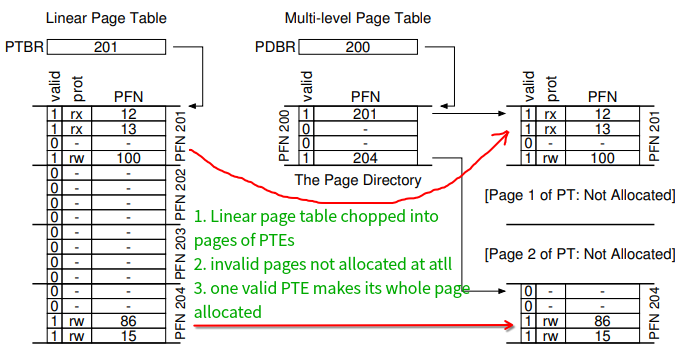
\includegraphics[width=\linewidth]{imgs/multi_level_pt}
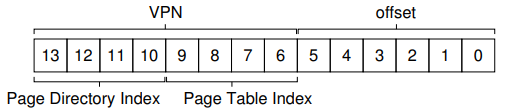
\includegraphics[width=\linewidth]{imgs/two_level_pt}
\begin{enumerate}
\item \texttt{PDEAddr = PageDirBase + (PDIndex * sizeof(PDE))}
\item \texttt{PTEAddr = PDE.PFN << SHIFT + (PTIndex * sizeof(PTE))}
\item \texttt{PhysAddr = (PTE.PFN << SHIFT) + offset}
\end{enumerate}
\begin{minipage}{.5\linewidth}
  \flushleft
  \begin{itemize}
  \item Space usage in proportion to in-use addr space
  \item each portion of PT can fit neatly within a page $\to$ \textbf{easier} memory management: OS grabs next free page for alloc or grow
  \end{itemize}
\end{minipage}
\begin{minipage}{.5\linewidth}
  \flushleft
  \begin{itemize}
  \item on TLB miss $\to$ two loads from memory (slower)
  \item \textbf{complexity}$\uparrow$ (hardware or OS) of handling page-table lookup (on TLB miss).
  \end{itemize}
\end{minipage}
